\presec
\section{The \fname~Technique} \postsec

In this section, we present the details of our \fname~technique which can be applied to all exisiting sketches.
We mainly present two key techniques of our \fname: \textit{unbalanced parameter setting and overflow skip}.
By applying the unbalanced parameter setting technique, we can increase the width of arrays with a small counter size, which can significantly reduce the probability of hash collisions.
Therefore, the overall accuracy can be improved. %and thus significantly enhance the accuracy of \texttt{cold items}.
%By applying the overflow skip technique, we can guarantee the accuracy of \texttt{hot items} keeping at a high level.
By applying the overflow skip technique, we can prevent the illogical results for some items.
Table \ref{table:symbols} summarizes the symbols and abbreviations used in this paper.

\begin{table}[htbp]
	\centering
	\caption{Symbols \& abbreviations used in the paper}
	\begin{tabular}{|c|l|}
		\hline
		\textbf{Symbol}&\textbf{Description}\\
		\hline
		$d$& \# of arrays of a sketch\\
		\hline
		$w_i$& \# of counters in the $i^{th}$ array\\
		\hline
		$\overline{w}_i$& \# of bits in the $i^{th}$ array\\
		\hline
		$b_i$& the counter size in the $i^{th}$ array\\
		\hline
		$e$& an arbitrary element\\
		\hline
		A$_i$& the $i^{th}$ array in a sketch\\
		\hline
		A$_i$[$j$]& the counter in the $j^{th}$ position of the $i^{th}$ array\\
		\hline
		$h_i(.)$& the $i^{th}$ hash function\\
		\hline
		CR& the correct rate of a sketch\\
		\hline
		RE& the relative error of an item\\
		\hline
		AE& the absolute error of an item\\
		\hline
		ARE& the average relative error of a sketch\\
		\hline
		AAE& the average absolute error of a sketch\\
		\hline
		Mips& mega-instructions per second\\
		\hline
	\end{tabular} 
	\label{table:symbols}
\end{table}

\presub
\subsection{Technique I: Unbalanced Parameter Setting} \postsub

\presub
\subsubsection{Rationale} \postsub

As stated above, in most real datasets, most items have a small frequency (typically less than 10), and only a few items have a large frequency. 
%Prior approaches mainly focus on \texttt{hot items}, and achieve higher accuracy of these items. Here we claim that \texttt{cold items} are also important, since the percentage of \texttt{cold items} is much larger than that of \texttt{hot items}.
Conventional sketches use the same parameters for each array, but this parameter setting could wastes a lot of memory since most items have a small frequency, while the counter size should be large enough to contain the largest frequency among all items in the data stream.
Therefore, with fixed memory size, the width of each array can be quite small, and thus more hash collisions will happen, leading to a low overall accuracy.
%Therefore, we should use different parameters for different arrays.
So using different parameters for different arrays is a wise solution.
On the one hand, we can set a smaller counter size for some arrays, and thus we can also set a larger width for these arrays.
It can significantly reduce the probability of hash collisions for these arrays, and therefore improve the arruacy.
On the other hand, we should also set a big counter size for some other arrays, since we should have counters whose size is big enough to contain large frequencies.
Furthermore, the width of these arrays do not need to be large, since the percentage of items with large frequencies is small.
Therefore, it can also guarantee the accuracy of \texttt{hot items}.
Sketches using our unbalanced parameter setting technique may take on different structures. Here we mainly introduce two versions of our technique.

\presub
\subsubsection{Version 1} \postsub

Based on conventional sketches like CM sketches, we first set different counter sizes for different arrays in the first version.

\noindent\textbf{Technical content: }As the name of our technique indicates, the first version of our technique uses the idea of cell division.
There are two main points to present this version: 1) it uses the same amount of memory (same number of bits) for each array, like conventional sketches; 2) it uses different counter size for each array. For example, there are 4 arrays in a sketch, and it uses a counter size of 2 bits, 4 bits, 8 bits and 16 bits for the 4 arrays. Therefore, if the width of the fourth array is $w$, then the first three arrays has a width of $8w$, $4w$, and $2w$, respectively.
Assume that each counter is a cell, and each division will transform one single bigger cell into two smaller cells.
Then counters in the first array have experienced cell division for three rounds, and those in the second and the third array have experienced for two rounds and one round, respectively. Furthermore, the total number of bits keeps constant after each round of division, which resembles the substance conservation phenomenon in cell divisions.
The structure of this example is shown in Figure \ref{draw:version1}.

\noindent\textbf{Analysis: }As stated above, arrays with a small counter size reduces the probability of hash collisions, and thus increase the accuracy significantly. Arrays with a large counter size is able to contain the large item frequencies, and can prevent large errors for items with large frequencies. Therefore, the overall accuracy of the data stream can be enhanced greatly. However, this parameter setting for sketches may not be the best in many cases.
Assume that there are only about 10\% \texttt{cold items} whose frequency is less than 3, then most counters in the array whose counter size is 2 bits will overflow. It will waste a large amount of memory usage, and the performance is not good enough.
In the next version, we will solve this issue by differentiate another parameter among different arrays. 

\begin{figure}[htbp]
	\centering
	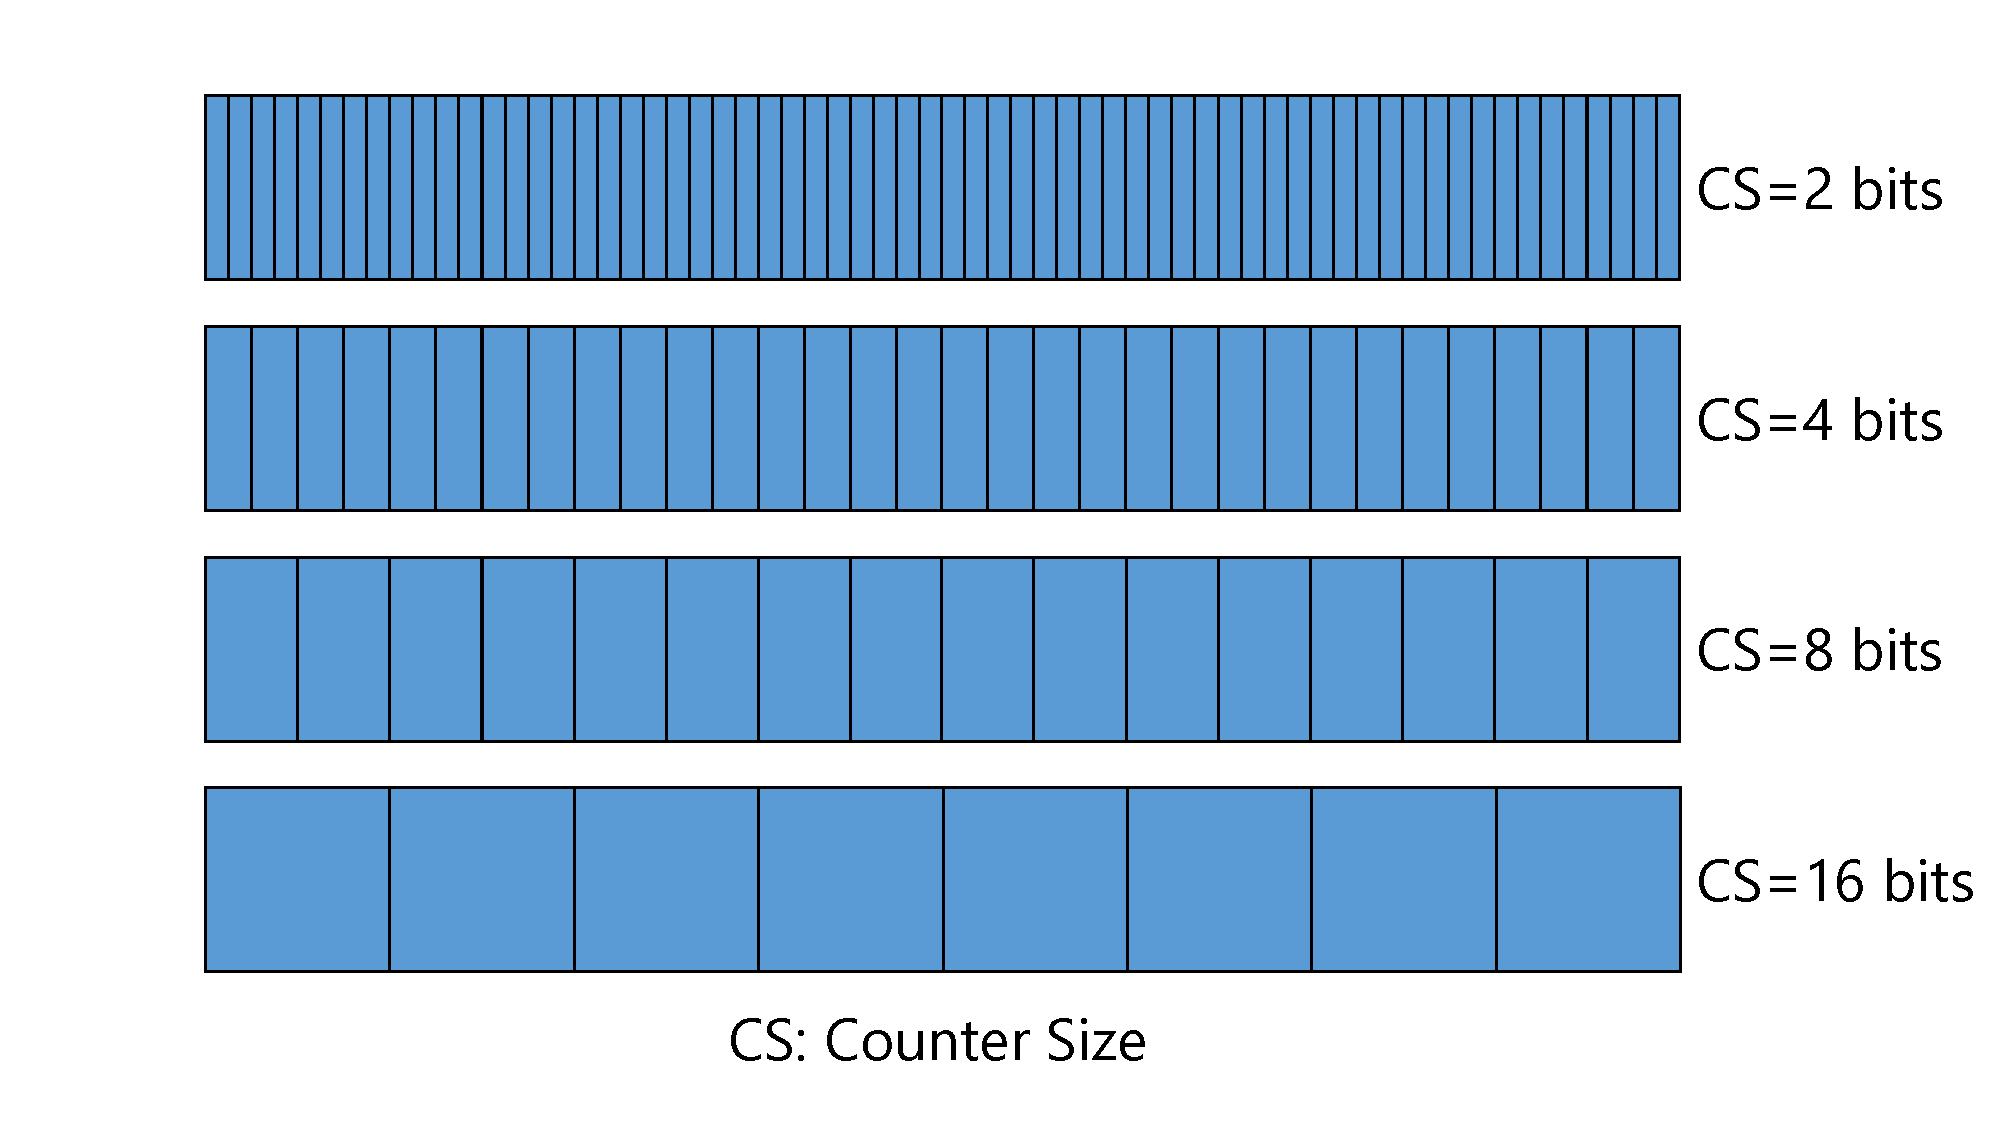
\includegraphics[width=3.5in]{cdv1}
	\caption{The structure of a sketch using the first version of \fname.} 
	\label{draw:version1}
\end{figure}

\presub
\subsubsection{Version 2} \postsub

Based on the first version of our unbalanced parameter setting technique, we can make further improvements on other parameters.
As mentioned above, the distribution of item frequencies will affect the performance of the first version of unbalanced parameter setting technique greatly.
Therefore, we should also take the parameter width into account.

\noindent\textbf{Technical content: }For different distributions of item frequencies, there are different suitable parameter settings. If the percentage of \texttt{cold items} decreases, the width of arrays with small counter size should decrease, and accordingly the width of arrays with larger counter size should increase. If that percentage increases, then the width of arrays with small counter size should increase, and that of arrays with larger counter size should decrease.
Therefore, we should allocate different widths for different arrays based on the distribution.
For example, as shown in Figure \ref{draw:version2}, there are 4 arrays in a sketch, and these 4 arrays have a counter size of 2 bits, 4 bits, 8 bits and 16 bits, respectively.
When the degree of nonuniformity of the dataset is high, then the total number of bits in the first array increases while that in the last array becomes smaller.
When the degree of nonuniformity is small, then the total number of bits in the last array increases.
It resembles cell proliferation and cell apoptosis: when there are enough nutrition, cells will proliferate; and when lack of nutrition, some cells will die.
\textit{The key point of this technique is to use the nonuniformity of past data streams to determine the parameter settings.}

\begin{figure}[htbp]
	\centering
	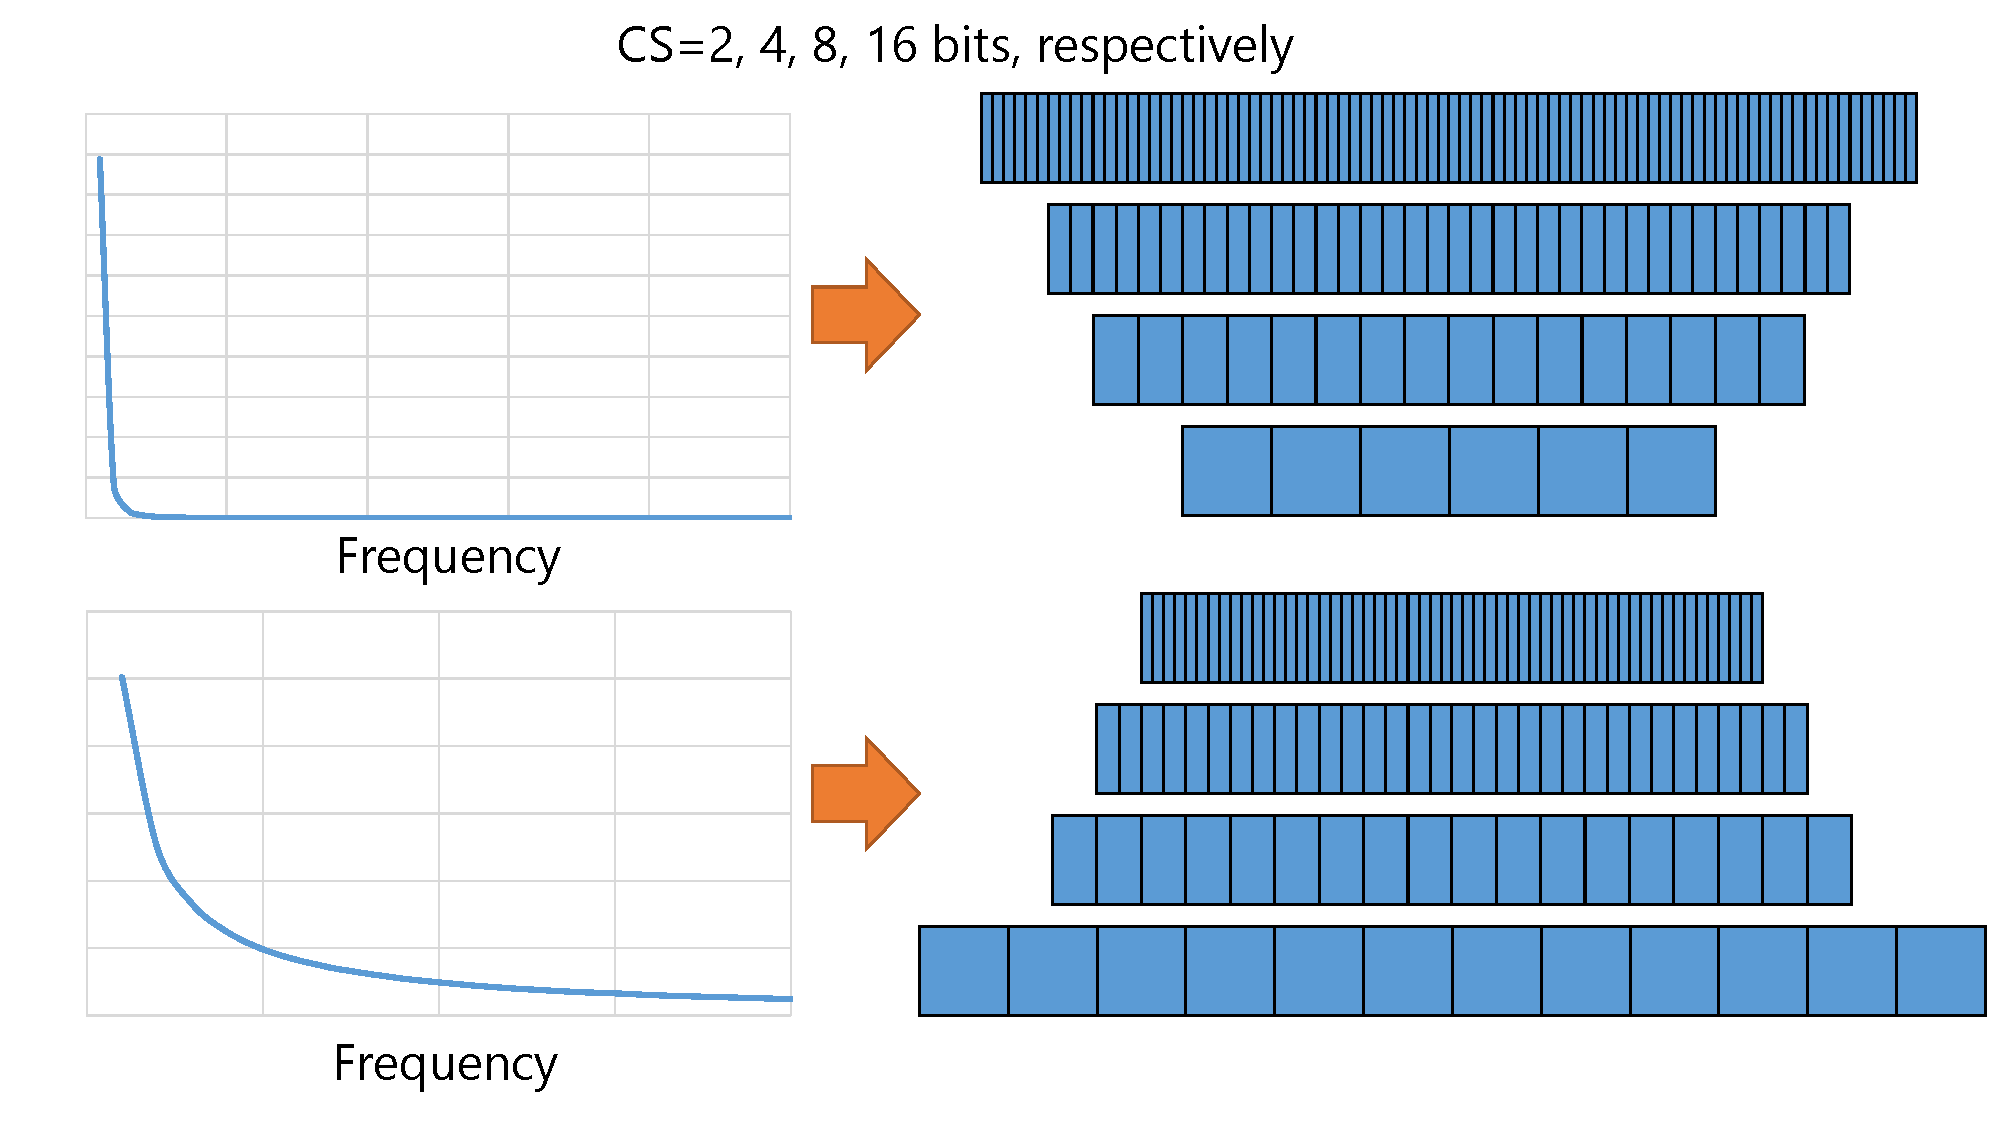
\includegraphics[width=3.5in]{cdv2}
	\caption{The structure of a sketch using the second version of \fname.} 
	\label{draw:version2}
\end{figure}


\noindent\textbf{Analysis: }This version of unbalanced parameter setting can fit the distribution of data streams, so that it can almost achieve the best accuracy as long as there are no drastically changes in the distribution.
However, there is still another problem unsolved.
This version cannot handle counter overflows properly which can lead to low accuracy, especially for \texttt{hot items}.
To address this problem, we propose our second technique in the next part.

\presub
\subsection{Technique II: Overflow Skip} \postsub

In this part, we present our second technique, named \textit{Overflow Skip}.
This technique is aimed to handle counter overflows properly in order to prevent low accuracy for \texttt{hot items}.
If we simply use the same query algorithms as conventional sketches like CM sketches, we will get illogical results.
For example, if we are using a CM sketch with 4 arrays as mentioned above, and there is an item $e$ has a frequency of 10000. The item $e$ is mapped to 4 counters in the sketch, \ie, $A_1[h_1(e)] \dots A_4[h_4(e)]$. When querying the item $e$, we should report the minimum value of these 4 counters. However, the counter $A_1[h_1(e)]$ has a size of only 2 bits, and thus the value in this counter is only 3 due to the counter overflow.
Therefore, we will get an estimated frequency of 3.
Obviously, it is illogical and leads to huge errors.
To address this problem, we use Overflow Skip technique to handle overflows.
\textit{When querying an item, we will get $d$ mapped counters, where $d$ represents the number of arrays in a sketch. If a counter overflows, we will treat the counter as a flag instead of a meaningful frequency, and omit its value when reporting the minimum value among all these $d$ counters.}
For example, as shown in Figure \ref{draw:os}, we are using a CM sketch width 4 arrays as mentioned before.
When querying an item $e$, it is mapped to 4 counters with values of 3, 15, 18 and 41.
As the first counter and the second counter overflow, their values are omitted.
Therefore, we report the estimated frequency of 18 instead of 3.
The pseudocode of this technique applying to the CM sketch is presented in Algorithm \ref{alg:os}.

\begin{figure}[htbp]
	\centering
	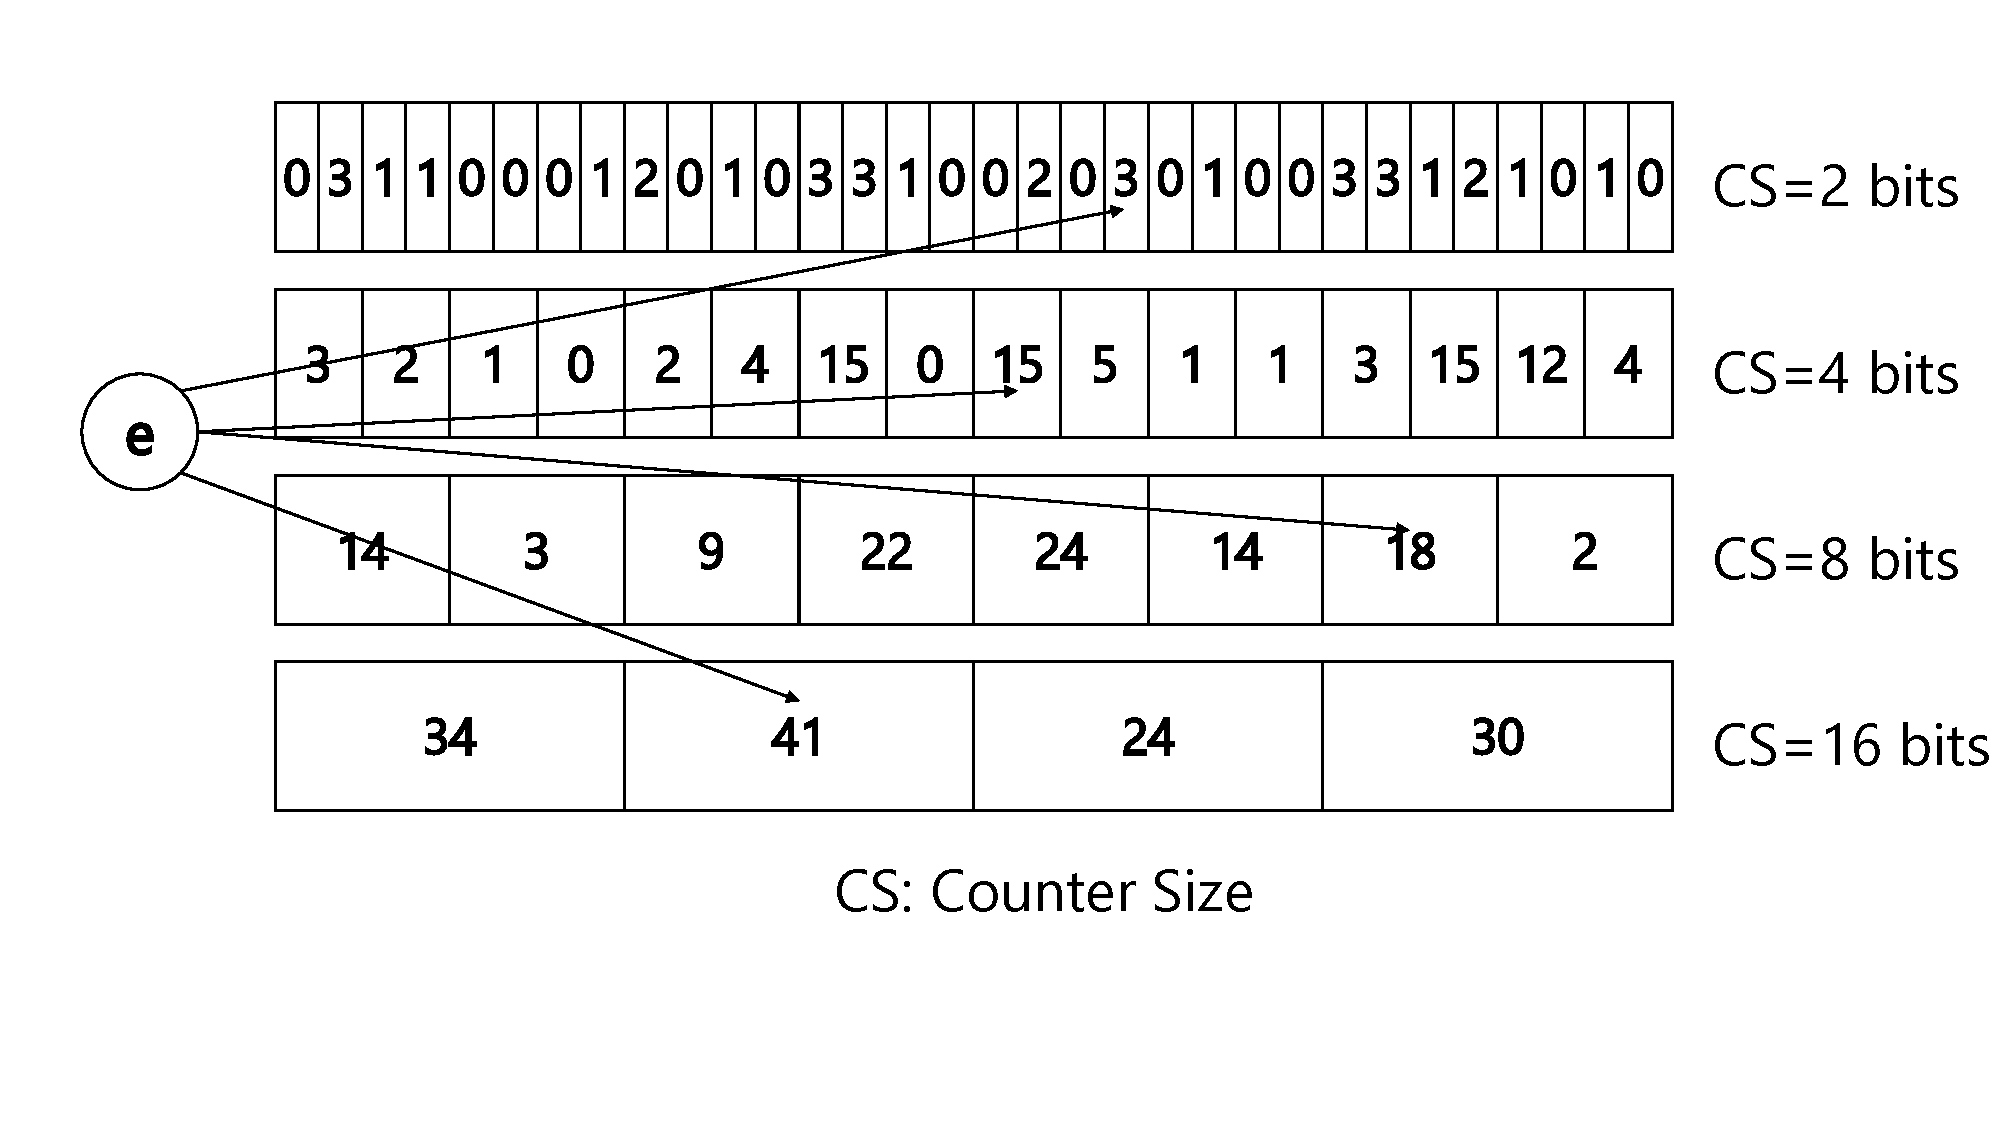
\includegraphics[width=3.5in]{os}
	\caption{The overflow skip technique.} 
	\label{draw:os}
\end{figure}

\begin{algorithm}[h]
	\caption{Query process using the overflow skip technique}
	\label{alg:os}
	% \begin{algorithmic}[1]
	% \Require
	\KwIn{ $e$: an arbitrary item; $A$: a CM sketch; $b$: the counter size of each array}
	% \Ensure
	\KwOut{The estimated frequency of $e$}
%	Procedure {$Query$($e$, $A$)}
	
	$min=MAX\_VALUE$\;
	\For{$j=1$,$j \leqslant d$, $j++$}
	{
		\If{$A_i[h_i(e)]<2^{b_i}-1$}
		{
			\If{$min>A_i[h_i(e)]$}
			{
				$min=A_i[h_i(e)]$\;
			}
		}
	}
	return $min$\;
%	$min=MAX\_VALUE$\;
%	\For{$i=1$;$i\leqslqnt d$;$i++$}
%	{
%		\If{$A_i[h_i(e)]$ overflows}
%		{
%			continue\;
%		}
%	}
\end{algorithm}

\presub
\subsection{Cost Analysis} \postsub

In this part, we give a brief analysis to prove that our \aname~technique is free of extra costs.

\noindent\textbf{Memory access: }For a CM sketch without using our technique, the number of memory accesses for each insertion process or each query process is $d$, the number of arrays in the sketch. After using our \aname~technique, it also requires $d$ memory accesses for each insertion and query process, since each counter can be accessed with one single memory access even if the counter size varies from different arrays. Therefore, there are no extra memory access for CM sketches after using our technique.
This conclusion can also be applied to other sketches, whose analysis is omitted due to space limitation.

\noindent\textbf{Computational complexity: }Except for the amount of computations needed for sketches without using our technique, sketches using our technique requires at most 2 displacement operations for each mapped counter when performing insertion or query processes.
This extra amount of computations is far smaller than that required before using our technique, including hash function computations.
Therefore, our \aname~technique almost introduce no extra computational complexity.

\noindent\textbf{Others: }Our \aname~technique also does not introduce other extra costs. For example, the CM sketch and the CU sketch suffer from no under-estimation errors, and so do these sketches after using our technique. The proof of this will be presented in the next section.
Furthermore, the CM sketch after using our technique also supports deletion operations like those without using our technique.